\documentclass[tikz,border=2pt]{standalone}
\usepackage{amsmath,amssymb}
\usetikzlibrary{arrows.meta,positioning}

\definecolor{upperblue}{HTML}{2F6E9E}
\definecolor{upperfill}{HTML}{EAF3F8}
\definecolor{lowerorange}{HTML}{B8612B}
\definecolor{lowerfill}{HTML}{FBEFE7}
\definecolor{feedbackgray}{HTML}{5C6670}

\begin{document}
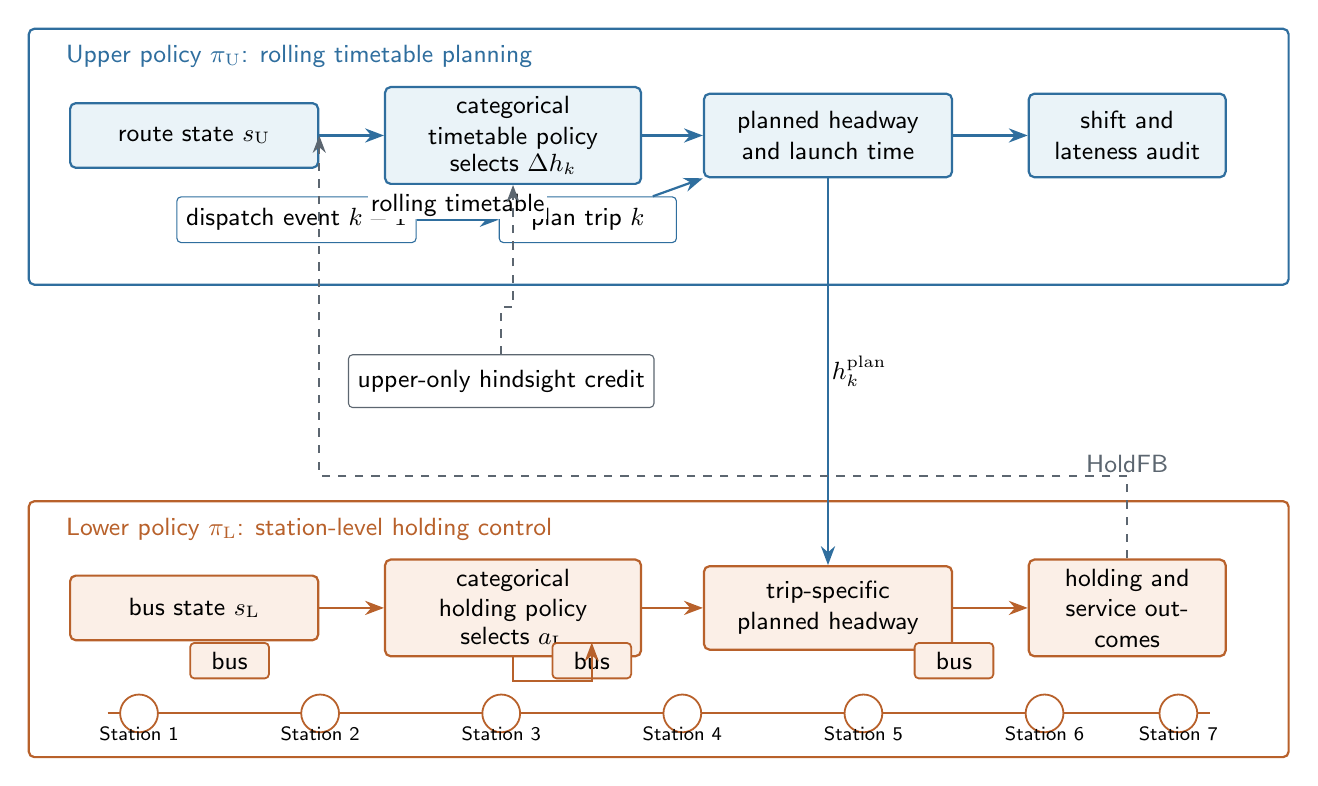
\begin{tikzpicture}[
  x=1cm,
  y=1cm,
  font=\sffamily\small,
  >=Stealth,
  frame/.style={rounded corners=2pt, line width=0.8pt},
  upperbox/.style={frame, draw=upperblue, fill=upperfill},
  lowerbox/.style={frame, draw=lowerorange, fill=lowerfill},
  signal/.style={-{Stealth[length=2.4mm]}, line width=0.8pt},
  feedback/.style={-{Stealth[length=2.2mm]}, dashed, draw=feedbackgray, line width=0.75pt},
  station/.style={circle, minimum size=4.8mm, inner sep=0pt, draw=lowerorange, fill=white, line width=0.65pt},
  bus/.style={rounded corners=1.5pt, minimum width=10mm, minimum height=4.5mm, inner sep=1.2pt, draw=lowerorange, fill=lowerfill, line width=0.65pt}
]

\node[frame, draw=upperblue, minimum width=16.0cm, minimum height=3.25cm] (upperframe) at (8,4.15) {};
\node[anchor=west, text=upperblue] at (0.35,5.42) {Upper policy $\pi_{\mathrm U}$: rolling timetable planning};
\node[upperbox, minimum width=3.15cm, minimum height=0.82cm, align=center] (ustate) at (2.1,4.42) {route state $s_{\mathrm U}$};
\node[upperbox, minimum width=3.25cm, minimum height=1.06cm, text width=3.0cm, align=center] (upolicy) at (6.15,4.42) {categorical\\timetable policy\\[-1pt]selects $\Delta h_k$};
\node[upperbox, minimum width=3.15cm, minimum height=1.06cm, text width=2.9cm, align=center] (uplan) at (10.15,4.42) {planned headway\\and launch time};
\node[upperbox, minimum width=2.50cm, minimum height=1.06cm, text width=2.25cm, align=center] (uaudit) at (13.95,4.42) {shift and\\lateness audit};
\draw[signal, draw=upperblue] (ustate) -- (upolicy);
\draw[signal, draw=upperblue] (upolicy) -- (uplan);
\draw[signal, draw=upperblue] (uplan) -- (uaudit);

\node[draw=upperblue, fill=white, rounded corners=1.5pt, minimum width=2.35cm, minimum height=0.58cm, align=center] (dispatch) at (3.40,3.35) {dispatch event $k-1$};
\node[draw=upperblue, fill=white, rounded corners=1.5pt, minimum width=2.25cm, minimum height=0.58cm, align=center] (nexttrip) at (7.10,3.35) {plan trip $k$};
\draw[signal, draw=upperblue] (dispatch) -- node[above, fill=white, inner sep=1pt] {rolling timetable} (nexttrip);
\draw[signal, draw=upperblue] (nexttrip) -- (uplan.south west);

\node[draw=feedbackgray, fill=white, rounded corners=1.5pt, minimum width=3.1cm, minimum height=0.67cm, align=center] (credit) at (6.0,1.30) {upper-only hindsight credit};
\draw[feedback] (credit.north) -- ++(0,0.6) -| (upolicy.south);

\node[frame, draw=lowerorange, minimum width=16.0cm, minimum height=3.25cm] (lowerframe) at (8,-1.85) {};
\node[anchor=west, text=lowerorange] at (0.35,-0.58) {Lower policy $\pi_{\mathrm L}$: station-level holding control};
\node[lowerbox, minimum width=3.15cm, minimum height=0.82cm, align=center] (lstate) at (2.1,-1.58) {bus state $s_{\mathrm L}$};
\node[lowerbox, minimum width=3.25cm, minimum height=1.06cm, text width=3.0cm, align=center] (lpolicy) at (6.15,-1.58) {categorical\\holding policy\\[-1pt]selects $a_{\mathrm L}$};
\node[lowerbox, minimum width=3.15cm, minimum height=1.06cm, text width=2.9cm, align=center] (ltarget) at (10.15,-1.58) {trip-specific\\planned headway};
\node[lowerbox, minimum width=2.50cm, minimum height=1.06cm, text width=2.25cm, align=center] (outcomes) at (13.95,-1.58) {holding and\\service outcomes};
\draw[signal, draw=lowerorange] (lstate) -- (lpolicy);
\draw[signal, draw=lowerorange] (lpolicy) -- (ltarget);
\draw[signal, draw=lowerorange] (ltarget) -- (outcomes);

\draw[signal, draw=upperblue] (uplan.south) -- node[right, fill=white, inner sep=1pt] {$h_k^{\mathrm{plan}}$} (ltarget.north);
\draw[feedback] (outcomes.north) -- ++(0,1.05) node[above, fill=white, inner sep=1pt, text=feedbackgray] {HoldFB} -| (ustate.east);

\draw[draw=lowerorange, line width=0.7pt] (1.0,-2.92) -- (15.0,-2.92);
\foreach \x/\name in {1.4/1,3.7/2,6.0/3,8.3/4,10.6/5,12.9/6,14.6/7} {
  \node[station] at (\x,-2.92) {};
  \node[below=1.5pt] at (\x,-2.92) {\scriptsize Station \name};
}
\node[bus] at (2.55,-2.25) {bus};
\node[bus] at (7.15,-2.25) {bus};
\node[bus] at (11.75,-2.25) {bus};
\draw[signal, draw=lowerorange] (lpolicy.south) -- ++(0,-0.3) -| (7.15,-2.02);

\end{tikzpicture}
\end{document}
